\documentclass[aspectratio=169]{ctexbeamer}
\usepackage[T1]{fontenc}
\usepackage{latexsym,amsmath,xcolor,multicol,booktabs,calligra}
\usepackage{graphicx,listings,stackengine}
\usepackage{hyperref}

\usepackage{PekingU}

% 去掉每节/子节前面的自动目录页
\AtBeginSection[]{}
\AtBeginSubsection[]{}

% ===== 每节课改这里 =====
\author{Cap1taL}
\title{模拟赛2讲解}
\subtitle{さあ……始めましょう}
\date{2026年8月}
% ========================

% 代码高亮设置
\definecolor{deepblue}{rgb}{0,0,0.5}
\definecolor{deepred}{rgb}{0.6,0,0}
\definecolor{deepgreen}{rgb}{0,0.5,0}
\definecolor{halfgray}{gray}{0.55}

\lstset{
    basicstyle=\ttfamily\small,
    keywordstyle=\bfseries\color{deepblue},
    emphstyle=\ttfamily\color{deepred},
    stringstyle=\color{deepgreen},
    numbers=left,
    numberstyle=\small\color{halfgray},
    rulesepcolor=\color{red!20!green!20!blue!20},
    frame=shadowbox,
}

\begin{document}

\kaishu

% 封面
\begin{frame}
    \titlepage
\end{frame}

% 目录
% \begin{frame}{目录}
%     \tableofcontents[sectionstyle=show,subsectionstyle=show/shaded/hide,subsubsectionstyle=show/shaded/hide]
% \end{frame}

% ===== 从这里开始写你的内容 =====

\begin{frame}{Who is Misumi Uika……Hatsune?}
    % 整行居中布局
    \centering
    \begin{minipage}{0.8\textwidth}
    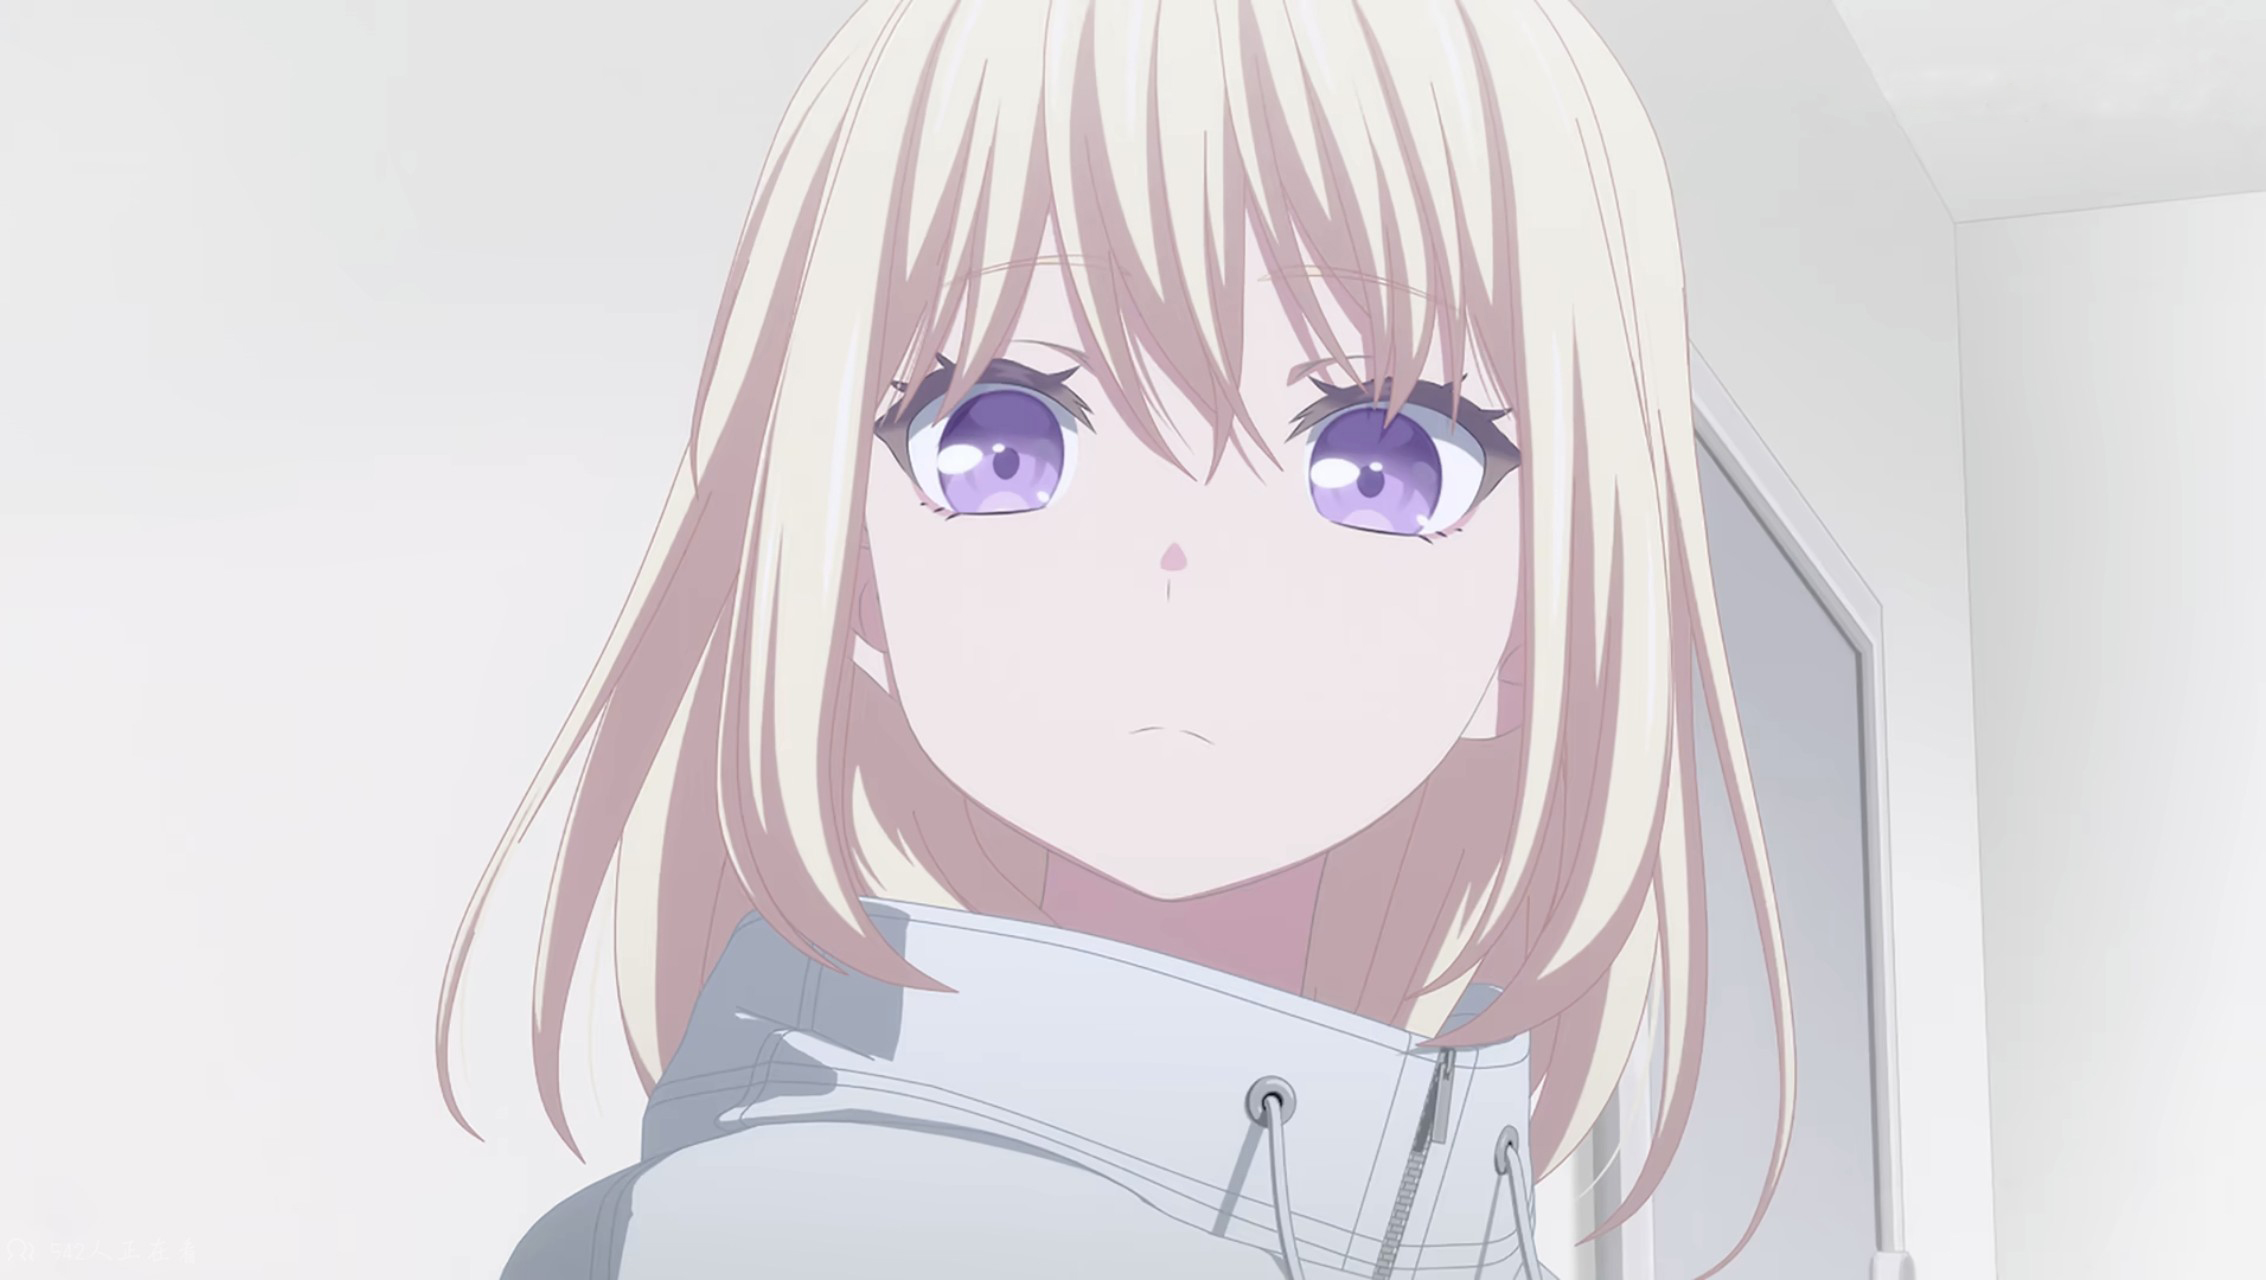
\includegraphics[width=\linewidth]{pic/1.jpg}
    \end{minipage}
\end{frame}

\section{Sakiko的乘积}

\subsection{Sakiko的乘积}
\begin{frame}{题意}
    求等差序列的积，对 $1145141$ 取模。多组测试数据。

    $d,n,a\le 10^9,T\le 10^4$
\end{frame}

\begin{frame}{Solution}
    \begin{itemize}
        \item 分类讨论题
        \item $n\le 50$ 的部分分给暴力实现，与正解关系不大
        \item 我们首先将 $a,d$ 对 $mod$ 取模，显然这不会改变答案
        \item 若 $d=0$，则答案就是 $a^n$，快速幂直接输出即可
        \item 若 $a=0$ 或 $n\ge mod$，则必定会有为 $ 0 $ 的项，输出 $0$
        \item 现在我们判掉了一些边界情况 
    \end{itemize}
\end{frame}

\begin{frame}{Solution}
    \begin{itemize}
        \item 考虑 $d=1$ 的情况，我们的答案一定形如一些数连乘。具体的，答案应该为 $\frac{(a+n-1)!}{(a-1)!}$
        \item 因此，在判断 $a+n-1$ 是否 $\ge mod$ 之后，我们就可以预处理 $mod$ 以内的阶乘及其逆元，$O(1)$ 计算答案。
        \item 现在来考虑 $d\neq 1$ 的情况。自然而然的，我们希望把它变回 $d=1$ 的情况。
        \item 注意到 $1145141$ 是一个质数，因此分数在模意义下一定是可以处理的。
        \item 我们将这个等差数列的每一项均除以 $d$，变回公差为 $ 1 $ 的情况，按照 $d=1$ 的方法去做，最后再对答案乘 $d^n$ 即可。
    \end{itemize}
\end{frame}

\section{Uika 的删除}
\subsection{Uika 的删除}
\begin{frame}{题面}
    一个序列，初始 $a_i=i$，每次你可以挑选一个长度为 $k$ 的子序列，删除除了中位数之外的所有数。问能否变为 $b$ 序列

    $n,k\le 2\times 10^6$，$k$ 为奇数。
\end{frame}

\begin{frame}{Solution}
    \begin{itemize}
        \item 很明显每次删除的元素数量是一定的，为 $k-1$，因此如果删除数量不是其倍数，则无解
        \item 结论：只要我们可以找到一个位置，做最后一次删除，则答案为 YES。
    \end{itemize}
\end{frame}

\begin{frame}{Solution}
    \begin{itemize}
        \item “中位数”很特殊，不好下手，想办法从相对确定的情况下手
        \item 考虑最后一次删除，它的中位数一定被保留在 $b$ 中了。因此我们不妨在 $b$ 中找到它
        \item 记 $D=\frac{k-1}{2}$
        \item 若删除次数为 $ 1 $，则我们的结论显然正确
        \item 若删除次数大于 $ 1 $，则先考虑后两次删除，我们会删除 $4D$ 个元素，然后再进行归纳
        \item 最后删除的数字选择是随意的，我们总是可以选择恰当的数字 “撤销删除”，使得倒数第二次删除保留的“中位数”是我们最后一次删除的数字，或者与最后一次相同
    \end{itemize}
\end{frame}

\begin{frame}{Solution}
    \begin{itemize}
        \item 具体地，考虑这 $4D$ 个元素如何分布在我们选择的中心附近。
        \item 若刚好左侧 $2D$ 个右侧 $2D$ 个，我们只需要两次选择相同的中位数即可。
        \item 若有更多的元素位于左侧，我们在 $4D$ 个数字中选择 $[D+1,2D]$ 作为最后一次删除的数字
        \item 若有更多的元素位于右侧，我们在 $4D$ 个数字中选择 $[2D+1,3D]$ 作为最后一次删除的数字
        \item 容易证明按照如上规则操作，我们能一直维持 “最后一次操作存在” 的合法状态
    \end{itemize}
\end{frame}


\section{Mutsumi 的爱}
\subsection{Mutsumi 的爱}
\begin{frame}{题面}
    一个初始全 $ 0 $ 的序列，有 $m$ 次修改操作，每次操作给定 $x,y$，会多次把 $[1,x]$ 内的最小值加 $ 1 $，重复 $y$ 次。求出最终的序列

    $n,m\le 10^5,\; b_i\le 10^{12}$
\end{frame}

\begin{frame}{Solution}
    \begin{itemize}
        \item 考虑 $b_i=1$ 的特殊性质，每次操作是给前缀最小值加 $1$。暴力做法是 $O(nm)$，使用一些数据结构加速可以做到 $O(m\log n)$
        \item 上述做法难以推广到 $b_i>1$ 的情形，但通过观察 $b_i=1$ 的情况，我们能够发现，在这种规则下，我们的序列永远是单调不升的
        \item 有了单调性的限制，我们考虑一次修改，实际上会选择 $[l,x]$，将它区间推平为 $[v,v+1,\cdots,v+1,v,v,\cdots v]$ 的形式
        \item 我们尝试准确找到这样的区间
        \item 对于每个位置 $c_i$，检查 $c_i*(x-i+1)-\sum_{j=i}^x c_j$ 是否 $\le y$。我们要找到最小的 $i$ 满足上述不等式。这意味着 “$y$ 可以填平这个区间”
        \item 在填平之后，$y$ 还会剩下一些值。进行一些简单的运算，可以算出在 $c_i$ 的基础上又填充了多高，以及有多少位置是 $v+1$
    \end{itemize}
\end{frame}

\begin{frame}{Solution}
    \begin{itemize}
        \item 暴力执行刚才的操作是 O(nm) 的。
        \item 问题在于我们如何快速找到我们需要的最小左端点
        \item 注意到其合法与否满足单调性
        \item 可以使用线段树二分，只需要支持区间覆盖和区间和，复杂度 $O(m\log n)$
        \item 也可以暴力使用二分再套线段树查询，复杂度 $O(m\log^2 n)$，也可以通过
    \end{itemize}
\end{frame}


\section{Taki 的融合}
\subsection{Taki 的融合}
\begin{frame}{题面}
    给定数组 $a$。每次操作选择一个 $i$ 满足 $a_i=i$，删除 $a_i$ 和 $a_{i+1}$，剩余部分拼接。求最多操作次数。
    
    多组数据，$n,\sum n\le 800$
\end{frame}

\begin{frame}{Solution}
    \begin{itemize}
        \item $n$ 较小的测试点留给一些暴力做法
        \item 题目要求一个数只有 “落位” 到 $a_i=i$ 时才能成为我们删除的对象
        \item 不难感受到，由于序列越来越短，所有的数都在单向“向左移动”。可能有本来不能删除的数字归位，然后可以被删除
        \item 同时一个数需要“回落”的步骤也是固定的，为 $\frac{i-a[i]}{2}$
        \item 删除相邻+拼接，所以如果我们“匹配”同一步删除的数字，会形成类似括号序列的结构
        \item 结合数据范围，可以想到区间 DP
    \end{itemize}
\end{frame}

\begin{frame}{Solution}
    区间 DP
    \begin{itemize}
        \item 结合刚才的观察，我们知道删除前，需要一个“数字回落”的过程
        \item 对于 $n\le 100$，可以暴力固定这个回落进程。设 $f_{l,r,x}$ 表示在 $[l,r]$ 左侧删了 $x$ 个数，内部最多删几个数
        \item 转移只需要考虑 $l$ 与 $r$ 搭配删除（从 $f_{l+1,r-1,x}$ 转移），与内部分界的情况（从 $f_{l,k,x}$ 与 $f_{k+1,r,x+f_{l,k,x}}$）
        \item 复杂度 $O(n^4)$
    \end{itemize}
\end{frame}


\begin{frame}{Solution}
    区间 DP
    \begin{itemize}
        \item 上述做法难以直接优化，我们需要改变状态设计
        \item 思考上述转移本质上在做什么？转移二是平凡的，而转移一是在考虑区间内部能不能删空。
        \item 这启示我们不去做平凡的转移二。我们可以不再关注一个区间能删多少数，而是考虑一个区间被删空的情况。答案的计算只需要再进一步做线性 DP。
        \item 由此引出状态设计：$f_{l,r}$ 表示删空 $[l,r]$ 至少需要在 $[1,l-1]$ 删除多少个数
    \end{itemize}
\end{frame}


\begin{frame}{Solution}
    区间 DP
    \begin{itemize}
        \item 类似括号序列 (()) 和 ()()，显然有两种转移：
        \begin{itemize}
            \item 某一次删除了 $(a_l,a_r)$，这需要 $(l+1,r-1)$ 能先删空，直接转移即可
            \item 枚举断点，分别删空 $[l,k],[k+1,r]$。注意 $[k+1,r]$ 所需要的次数还有一部分由 $[l,k]$ 提供
            \item 转移形如两个数取 $\max$ 的形式
            \item 注意奇偶性细节带来的非法情况
        \end{itemize}
        \item 有了 $f_{l,r}$ 之后，我们就可以做一次线性 DP，设 $g_i$ 表示这个前缀最多操作多少次。枚举一个极长清空区间，转移时利用 $f_{l,r}$ 判断合法性
        \item 复杂度 $O(n^3)$
    \end{itemize}
\end{frame}





% ===== 结束页 =====

\begin{frame}
    \begin{center}
        {\Huge\calligra Thanks!}
    \end{center}
\end{frame}

\end{document}
